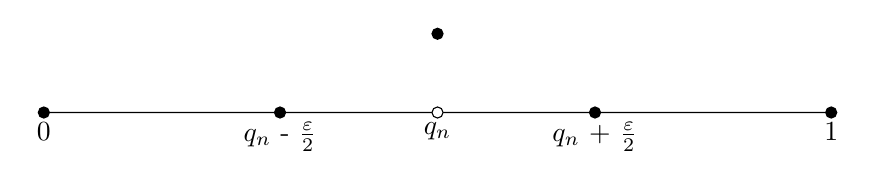
\begin{tikzpicture}
	% Punto (q,1)
	\filldraw (5,1) circle (2pt);	

	% Recta  y puntos
	\filldraw
	(0,0) circle (2pt) node[below]{0} --
	(3,0) circle (2pt) node[below]{$q_n$ - $\frac{\varepsilon}{2}$} --
	(7,0) circle (2pt) node[below]{$q_n$ + $\frac{\varepsilon}{2}$} --
	(10,0) circle (2pt) node[below]{1};
	
	% Recta de ceros
	\draw (0,0) -- (10,0);
	
	% Punto (q,0)
	\filldraw[color=white, draw=black] (5,0) circle (2pt) node[below, text=black]{$q_n$};	
\end{tikzpicture}